

\chapter{Asymmetrische Kryptosysteme}\label{ch:03}

\lstset{style=Python}

\section{Einführung}\label{sec:asymmetrischeKryptosysteme}

	Bei den Kryptosystemen, die wir im ersten Kapitel gesehen haben wurde jeweils derselbe Schlüssel zum Verschlüsseln wie zum Entschlüsseln verwendet. Diese Kryptosystem werden als \textbf{symmetrische} Kryptosysteme bezeichnet. Ein Problem bei symmetrischen Kryptosystemen ist, dass man häufig von der verschlüsselten Nachricht auf den Schlüssel schliessen kann. Dies erlaubt einem Angreifer das Kryptosystem zu knacken. Dies haben wir bereits bei den Kryptosystemen von Caesar und Vigenère gesehen.

	Bei einem \textbf{asymmetrischen Kryptosysteme}, oft auch \textbf{Public-Key-Kryptosystem} genannt, nutzt man ein Paar mathematisch verbundener Schlüssel. Einen öffentlichen Schlüssel (\textbf{Public-Key}), welche für jeden zugänglich ist, und eine privaten Schlüssel (\textbf{Private Key}), welcher geheim gehalten werden muss. 

	Man kann sich ein asymmetrisches Kryptosystem ein wenig so vorstellen wie einen Briefkasten an einem Haus. Es ist kein Geheimnis, wo sich der Briefkasten befindet. Jedoch genügt dieses Wissen einem Angreifer nicht, um Briefe, die in den Briefkasten geworfen werden, zu lesen. Nur der Besitzer des Briefkastens kann die Briefe dem Briefkasten entnehmen.

	Die Grundidee von einem asymmetrischen Kryptosystem lautet wie folgt:

	Alice und Bob generieren jeweils ein Schlüsselpaar, einen  öffentlichen Schlüssel (\emoji{unlock}), der von allen Personen gesehen und verwendet werden kann, und einen privaten Schlüssel (\emoji{key}), der nur im Besitz von Alice bzw. Bob ist. Wenn Alice eine Nachricht an Bob senden will, verwendet sie Bobs \textit{öffentlichen} Schlüssel, um die Nachricht zu verschlüsseln. Bob verwendet seinen \textit{privaten} Schlüssel zur Entschlüsselung, also den Schlüssel, auf den \textit{nur} er Zugriff hat (siehe \ref{fig:public-key-encryption}).Wichtig ist, dass die Nachricht die Alice an Bob schickt, mit dem öffentlichen Schlüssel nicht entschlüsselt werden kann. 

	\begin{figure}[H]
		\centering
		\begin{tikzpicture}[node distance = 1cm and 2cm, data/.style={rectangle, rounded corners, text width=3cm, minimum width=3cm, minimum height=1cm, text centered, draw=ForestGreen, fill=ForestGreen!30},
				startstop/.style={rectangle, rounded corners, minimum height=1cm, minimum width=3cm, text width=2.5cm, text centered, draw=RoyalBlue, fill=RoyalBlue!30}]

			\footnotesize
			% Nodes
			\node (plaintext) [data] {\emoji{woman-technologist} Alice};
			\node (ciphertext) [data, right=of plaintext] {Verschlüsselter\\Text};
			\node (publickey) [startstop, above=of ciphertext] {\emoji{unlock} Öffentlicher Schlüssel\\von Bob};

			\node (decryptedtext) [data, below=of ciphertext] {Verschlüsselter\\Text};
			\node (privatekey) [startstop, below=of decryptedtext] {\emoji{key} Privater Schlüssel\\ von Bob};
			\node (bob) [data, left=of decryptedtext] {\emoji{man-technologist} Bob};


			% Arrows
			\draw [->] (plaintext) -- (ciphertext);
			\draw [->] (ciphertext) -- (decryptedtext);
			\draw [->] (publickey) -- (ciphertext);
			\draw [->] (privatekey) -- (decryptedtext);
			\draw [->] (decryptedtext) -- (bob);

			\node at ($(plaintext.east)!0.5!(ciphertext.west)$) [above] {Klartext};
			\node at ($(publickey.south)!0.5!(ciphertext.north)$) [left] {Verschlüsselung};
			\node at ($(ciphertext.south)!0.5!(decryptedtext.north)$) [left] {Übertragung};
			\node at ($(privatekey.north)!0.5!(decryptedtext.south)$) [left] {Entschlüsselung};
			\node at ($(decryptedtext.west)!0.5!(bob.east)$) [above] {Klartext};
		\end{tikzpicture}
		\caption{Prinzip der Public-Key-Verschlüsselung}
		\label{fig:public-key-encryption}
	\end{figure}

	Das Diffie-Hellman-Merkel Protokoll, welches wir uns zuletzt angesehen haben, ist eine Public-Key-Kryptosystem. 

	\begin{myexercise}
		Was ist der Public-Key und was der Private Key bei Diffie-Hellman-Merkel?
		\begin{myanswer}
			Der Public Key ist für Alice und Bob gleich und besteht aus $(g,p)$. Alices Private Key ist $a$ und Bobs Private Key ist $b$.
		\end{myanswer}
	\end{myexercise}

	Ein asymmetrisches Kryptosystem kann auch verwendet werden, um die \textbf{Authentizität} einer Nachricht zu beweisen. D.h. Alice kann mit einem asymmetrischen Kryptosystem beweisen, dass die Nachricht tatsächlich von ihr und niemanden anderes stammt. Hierfür verschlüsselt Alice die Nachricht mit ihrem Private Key. Jede Person kann überprüfen, dass die Nachricht von Alice stammt, indem er oder sie Alices öffentlich zugänglichen Public Key verwendet, um die Nachricht wieder zu entschlüsseln. Da niemand ausser Alice den Private Key kennt, muss die Nachricht von Alice stammen. Dieses Verfahren wird auch als \textbf{Digitale Signatur} bezeichnet.

	Damit Bob am Ende wieder die entschlüsselte Nachricht erhält, muss der Private Key den Public Key rückgängig machen. In der Mathematik nennt man eine solche Funktion \textbf{Umkehrfunktion} oder \textbf{Inversfunktion}. 
	\begin{mydefinition}[Umkehrfunktion]
		Sei $f:A\rightarrow B$ eine Funktion. Die Funktion $g:B\rightarrow A$ ist die Umkehrfunktion von $F$ wenn
		\begin{align*}
			g(f(a)) = a hspace{0.5cm}\forall a\in A.
		\end{align*}
		Häufig schreibt man die Inversefunktion einer Funktion $f$ auch als $f^{-1}$. 
	\end{mydefinition}

	Ein asymmetrisches Kryptosystem kann theoretisch mit jeder invertierbaren Funktion ausgeführt werden. 

	\begin{myexercise}\label{ex:invertierbareFunktionen}
		Wählen Sie und Ihr Nachbar gemeinsam eine beliebige invertierbare Funktion $f$ aus und bestimmen Sie ihre Inverse $f^{-1}$. Verschlüsseln Sie nun jeder eine Nachricht, und senden Sie diese an Ihren Nachbarn. Entschlüsseln Sie danach die Nachricht, die Sie erhalten haben.
	\end{myexercise}

	In Aufgabe \ref{ex:invertierbareFunktionen} haben wir gezeigt, dass eine Menge Funktionen in Frage kommen, mit denen Alice und Bob ihre Nachrichten ver-/ bzw. entschlüsseln können. Da aber Eve ebenfalls den öffentlichen Schlüssel kennt, muss die Funktion, die dem asymmetrischem Kryptosystem zu Grunde liegt, so gewählt werden, dass Eve das Inverse nicht berechenen kann. 
	
	In der Mathematik nennen wir solche Funktionen \textbf{Einwegfunktionen}. Eine Einwegfunktion ist eine mathematische Funktion, die komplexitätstheoretisch „leicht“ berechenbar, aber „schwer“ umzukehren ist. Eine mathematische Einwegfunktion $F:X\rightarrow Y$ muss folgende Eigenschaften aufweisen:
	\begin{itemize}
		\item Man kann die Funktion $f(x)=y$ ``einfach'' \ berechnen; d.h. der Computer kann dies effizient. 
		\item Die Umkehrfunktion $f^{-1}(y)=x$ ist ``schwierig'' zu berechnen, und kann auch von einem Computer nicht effizient berechnet werden.
	\end{itemize}
	
	Jedes asymmetrische Kryptoverfahren verwendet eine Einwegfunktion für die Verschlüsselung. In \ref{sec:Diffie-Hellman-Merkel} haben wir bereits den diskreten Logarithmus als Einwegfunktion kennengelernt. Im nächsten Abschnitt lernen wir ein weiters asymmetrischen Kryptosystem kennen, welches auf dem \textbf{Faktorisierungsproblem} aufbaut. Das Faktorisierungsproblem ist die Aufgabe, eine gegebene Zahl in ihre Primfaktoren zu zerlegen. Derzeit ist keinen schnellen Algorithmus, welcher grosse Zahlen effizient in seine Primfaktoren zerlegen kann.

	Wichtig zu wissen ist, dass es für alle derzeit bekannten Einwegfunktionen derzeit keinen Beweis für die  Schwierigkeit ihrer Invertierung gibt. Das heisst, derzeit ist kein effizenter Algorithmus bekannt, der das Inverse der Einwegfunktion effizient bestimmt. Wir können aber auch nicht beweisen, dass dies wirklich der Fall ist. Sollte aber ein solcher Algorithmus gefunden werden, so ist jedes asymmetrische Kryptosystem, welches darauf aufbaut, hinfällig!


\section{RSA}\label{sec:RSA}

	Eines der auch heute am häufigsten benutzten asymmetrischen Kryptosysteme ist RSA, benannt nach seinen Erfindern Ron Rivest, Adi Shamir und Leonard Adleman. 

	\begin{figure}[H]
		\centering
		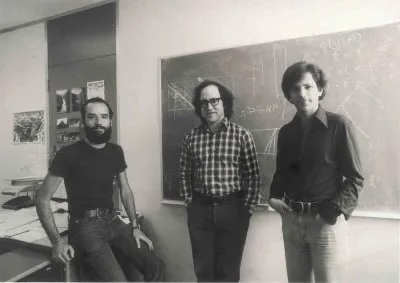
\includegraphics[width=0.7\linewidth]{Grundlagen_Info/03_Kryptologie/Figures/rsa.jpg}
		\caption{Ron Rivest, Adi Shamir und Leonard Adleman, die Erfinder des RSA-Verfahrens}
		\label{fig:rsa}
	\end{figure}

	Das RSA-Verfahren besteht aus folgenden Schritten:

	\begin{myprocedure}

		\begin{enumerate}
			\item \textbf{Schlüsselerzeugung:}
				\begin{itemize}
					\item Wählen Sie zwei (möglichst grosse) Primzahlen \( p \) und \( q \).
					\item Berechnen Sie das RSA-Modul \( n = p \cdot q \).
					\item Berechnen Sie die Eulersche Funktion \( \varphi(n) = (p-1)(q-1) \).
					\item Wählen Sie den \textit{Verschlüsselungsexponenten} \( e \), so dass dieser teilerfremd zu \( \varphi(n) \) und kleiner als $\varphi(n)$ ist. Dies bedeutet, dass der GGT von $e$ und $\varphi(n)$ 1 ist ($\operatorname{ggT}(e, \varphi(n)) = 1$).
					\item Berechnen Sie den \textit{Entschlüsselungexponenten} \( d \), so dass \( (e \cdot d) \mod \varphi(n) = 1  \) (privater Schlüssel). 
					\item Die Zahlen $p$, $q$ und $\varphi(n)$ werden nun nicht mehr benötigt und können gelöscht werden.
				\end{itemize}
			\item \textbf{Verschlüsselung:}
				\begin{itemize}
					\item Der Absender verschlüsselt eine \textbf{Klartext-Nachricht} \( \mathbf{m} \) (als Zahl) mit dem \textbf{öffentlichen Schlüssel} \( \mathbf{(e, n)} \):
							\[
								c = \mathbf{m}^e \mod n
							\]
					\item Das Ergebnis \( c \) ist der Kryptotext.
				\end{itemize}
			\item \textbf{Entschlüsselung:}
				\begin{itemize}
					\item Der Empfänger entschlüsselt die \textbf{verschlüsselte Nachricht} \( \mathbf{c} \) mit dem \textbf{privaten Schlüssel} \( \mathbf{(d, n)} \):
							\[
								\mathbf{m} = c^d \mod n
							\]
					\item Das Ergebnis \( \mathbf{m} \) ist die ursprüngliche Nachricht.
				\end{itemize}
		\end{enumerate}
	\end{myprocedure}


	\begin{myexample}
		Um den RSA Algorithmus besser zu verstehen, rechnen wir ein einfaches Beispiel mit kleinen Zahlen durch:
		\begin{enumerate}
			\item Wir wählen zwei (für diese Übung kleine) Primzahlen aus, \( p = 3 \) und \( q = 11 \). Daraus folgt:
				\begin{align*}
					n & = p \cdot q  \\
						& = 3 \cdot 11 \\
						& = 33
				\end{align*}
				\begin{align*}
					\varphi(n) & = (p-1)(q-1) \\
								& = 2 \cdot 10 \\
								& = 20
				\end{align*}
			\item Wir wählen \( e = 3 \), da \( \operatorname{ggT}(3, 20) = 1 \).
			\item Wir berechnen \( d \), so dass \( (e \cdot d) \mod \varphi(n) = 1  \) ergibt:
				\[
					(d \cdot 3) \mod 20 = 1  \quad \rightarrow \quad d = 7.
				\]
			\item Der öffentliche Schlüssel ist \( (e, n) = (3, 33) \), der private Schlüssel \( (d, n) = (7, 33) \).
		\end{enumerate}

		\textbf{Verschlüsselung:} Die Nachricht sei das Wort ``Code'', welches wir darstellen durch die Position der Buchstaben im Alphabet \( m = 3, 15, 4, 5 \). Berechnen Sie für jeden Buchstaben (hier nur für ``C'', also 3, gezeigt):
		\begin{align*}
			c & = m^e \mod n  \\
			& = 3^3 \mod 33 \\
			& = 27 \mod 33  \\
			& = 27.
		\end{align*}


		Der erste Buchstabe des Kryptotext wird also verschlüsselt als \( c = 27\).

		\textbf{Entschlüsselung:}
		\begin{align*}
			m & = c^d \mod n     \\
			& = 27^{7} \mod 33 \\
			& = 3
		\end{align*}

		Daraus ergibt sich \( m = 3 \), also die ursprüngliche Nachricht.
	\end{myexample}

	\begin{myexercise}
	Alice möchte eine Nachricht an Bob mit RSA verschlüsseln. Bob wählt die Hilfs-Primzahlen \( p = 5 \) und \( q = 7 \). Generieren Sie den öffentlichen Schlüssel ($e, n$) und den privaten Schlüssel ($d, n$) von Bob, indem Sie folgende Schritte ausführen:
	\begin{enumerate}
		\item Berechnen Sie \( n \) und \( \varphi(n) \).
		\item Sie wählen $e$ und $d$ aus.
	\end{enumerate}

	Verschlüsseln Sie nun die Nachricht \( m = 9 \) mit dem öffentlichen Schlüssel \( (e, n) \).

	Entschlüsseln Sie danach die verschlüsselte Nachricht \( c \) wieder mit dem privaten Schlüssel \( (d, n) \).
	\begin{myanswer}
		\begin{enumerate}
			\item \( n = p \cdot q = 5 \cdot 7 = 35 \), \( \varphi(n) = (p-1)(q-1) = 4 \cdot 6 = 24 \).
			\item Für $e$ können wir beispielsweise 5 wählen, da 5 teilerfremd mit 24 ist.
			\item \( (5 \cdot d) \mod 24 = 1\). Dies finden wir beispielsweise mit \( d = 5 \).
			\item Verschlüsselung:
			      \begin{align*}
				      c & = m^e\mod n\\
				        & = 9^5 \mod 35 \\
				        & = 4
			      \end{align*}.
			\item Entschlüsselung:
			      \begin{align*}
				      m & = c^d\mod n    \\
				        & =4^{5} \mod 35 \\
				        & = 9
			      \end{align*}
		\end{enumerate}
	\end{myanswer}
\end{myexercise}

Nehmen wir uns einen Moment Zeit, um zu verstehen, warum es so schwierig ist, das RSA Protokoll zu brechen: Wir wissen, dass $d\cdot e  \mod \varphi(n) = 1$. Das bedeutet, dass wenn Eve $\varphi(n)$ herausfindet, dann kann sie einfach $d$ bestimmen. 

Die Funktion $\varphi: \N_+\rightarrow \N_+$ auch Eulersche Phi-Funktion genannt, ist definiert als $\varphi(x) := \mid \{a\in\N | 1\leq a\leq x \wedge ggt(a,x) = 1\}\mid$. Das heisst, sie zählt die Anzahl natürlicher Zahlen, die teilerfremd zu $x$ sind. Für eine Primzahl $p$ ist es einfach zu sehen, dass $\varphi(p) = p-1$. Man kann auch zeigen, dass wenn $a$ und $b$ teilerfremd sind, dann gilt für $c=a\cdot b$ das $\varphi(c) = (a-1)(b-1)$. 

Im RSA Protokoll sind $p$ und $q$ Primzahlen und somit teilerfremd. Daher gilt $\varphi(n) = (p-1)(q-1)$. Die Zahl $n=p\cdot q$ ist Teil des öffentlichen Schlüssels und somit bekannt. Die Schwierigkeit des Faktorisierungsproblems besteht dadrin, dass es extrem schwierig ist, $p$ und $q$ herauszufinden, auch wenn $n$ bekannt ist. Auch können wir $\varphi(n)$ nur schwierig bestimmen, da wir dafür alle Teiler von $n$ kennen müssten.

\begin{myexercise}
	Versuchen Sie RSA zu brechnen. Der öffentliche Schlüssel $(e, n) = (7, 33)$. Die verschlüsselte Nachricht, die Sie erhalten, ist $29$. Was war die ursprüngliche Nachricht?
	\begin{myanswer}
		Wenn $n=33$, dann müssen $p=3$ und $q=11$ (oder umgekehrt) und $\varphi(n)= 20$. Um $d$ zu bestimmen lösen wir $7d\mod 20 = 1 \Rightarrow d = 3$ $m=29^{3} \mod 33 = 2$.
	\end{myanswer}
\end{myexercise}

\section{Lernziele Asymmetrische Kryptosysteme und RSA}

\begin{todolist}
  \item Ich weiss, was symmetrische und asymmetrische Kryptosysteme sind, und kenne mindestens zwei Beispiele für diese zwei Arten von Kryptosystemen.
  \item Ich weiss, wie man mit einem asymmetrischem Kryptosystem die Echtheit einer Nachricht beweisen kann.
  \item Ich weiss, was eine Einwegfuntkion ist, und ich kann erklären, warum asymmetrische Kryptosysteme Einwegfunktionen verwenden müssen. Ich kenne mindestens zwei Beispeiele für Einwegfunktionen.
  \item Ich weiss, wie das RSA Protokoll Funktioniert, und kann für gegebene $p$ und $q$ ein Schlüsselpaar erstellen.
\end{todolist}
